\subsubsection{Sequential switching between Tent and Logistic maps (SWITCH)} \label{sssec:switch}

SWITCH map is expressed as:

\begin{equation}
\begin{cases}
	x_{n+1}=
	\begin{cases}
		2x_n, & \mbox{if } 0\leq x_n\leq 1/2 \\
		2(1-x_n ), & \mbox{if } 1/2<x_n\leq 1
	\end{cases} \\
	x_{n+2}=4x_{n+1}(1-x_{n+1})
\end{cases}\label{eq:SWITCH}
\end{equation}
with $x_n\in\mathcal{R}$ and $n$ an even number.

Results with sequential switching are shown in Figs. \ref{fig:SWITCH_QuantiB} (a) to (f).
The entropy value calculated in floating point is $H_{val}=0.9722$, this value is slightly higher than the one obtained for the LOG map. 
For fixed point arithmetic this value is reached in $B=24$, but it stabilizes from $B=28$.
Regarding the ordering patterns the number of MP decreases to $586$, this value lower than the one obtained for LOG map.
It means the entropy $H_{BP}$ may increase up to $ln(134)/ln(720)\simeq 0.74$.
$BP$ and $BPW$ quantifiers reach their maximum of $H_{BP}=0.6546$ and $H_{BPW}=0.6313$ at $B=16$, but they stabilize from $B=24$.
Complexities are lower than for LOG, $C_{BP}=0.4580$ and $C_{BPW}=0.4578$, these values are reached for $B \geq 15$ but they are stable from $B \geq 23$.
Compared with LOG, statistical properties are better with less amount of bits, for $B \geq 24$ this map reaches optimal characteristics in the sense of random source.

\textcolor{red}{ESTO NO SE SI VA A IR EN LONG DOUBLE}
We can see some points with anomalies from $B \geq 49$ due to the same problem of LOG map, an multiplication needs double of precision to be done.
Furthermore, we encountred one initial condition in fixed point with an anomalous behaviour.

\begin{figure}
	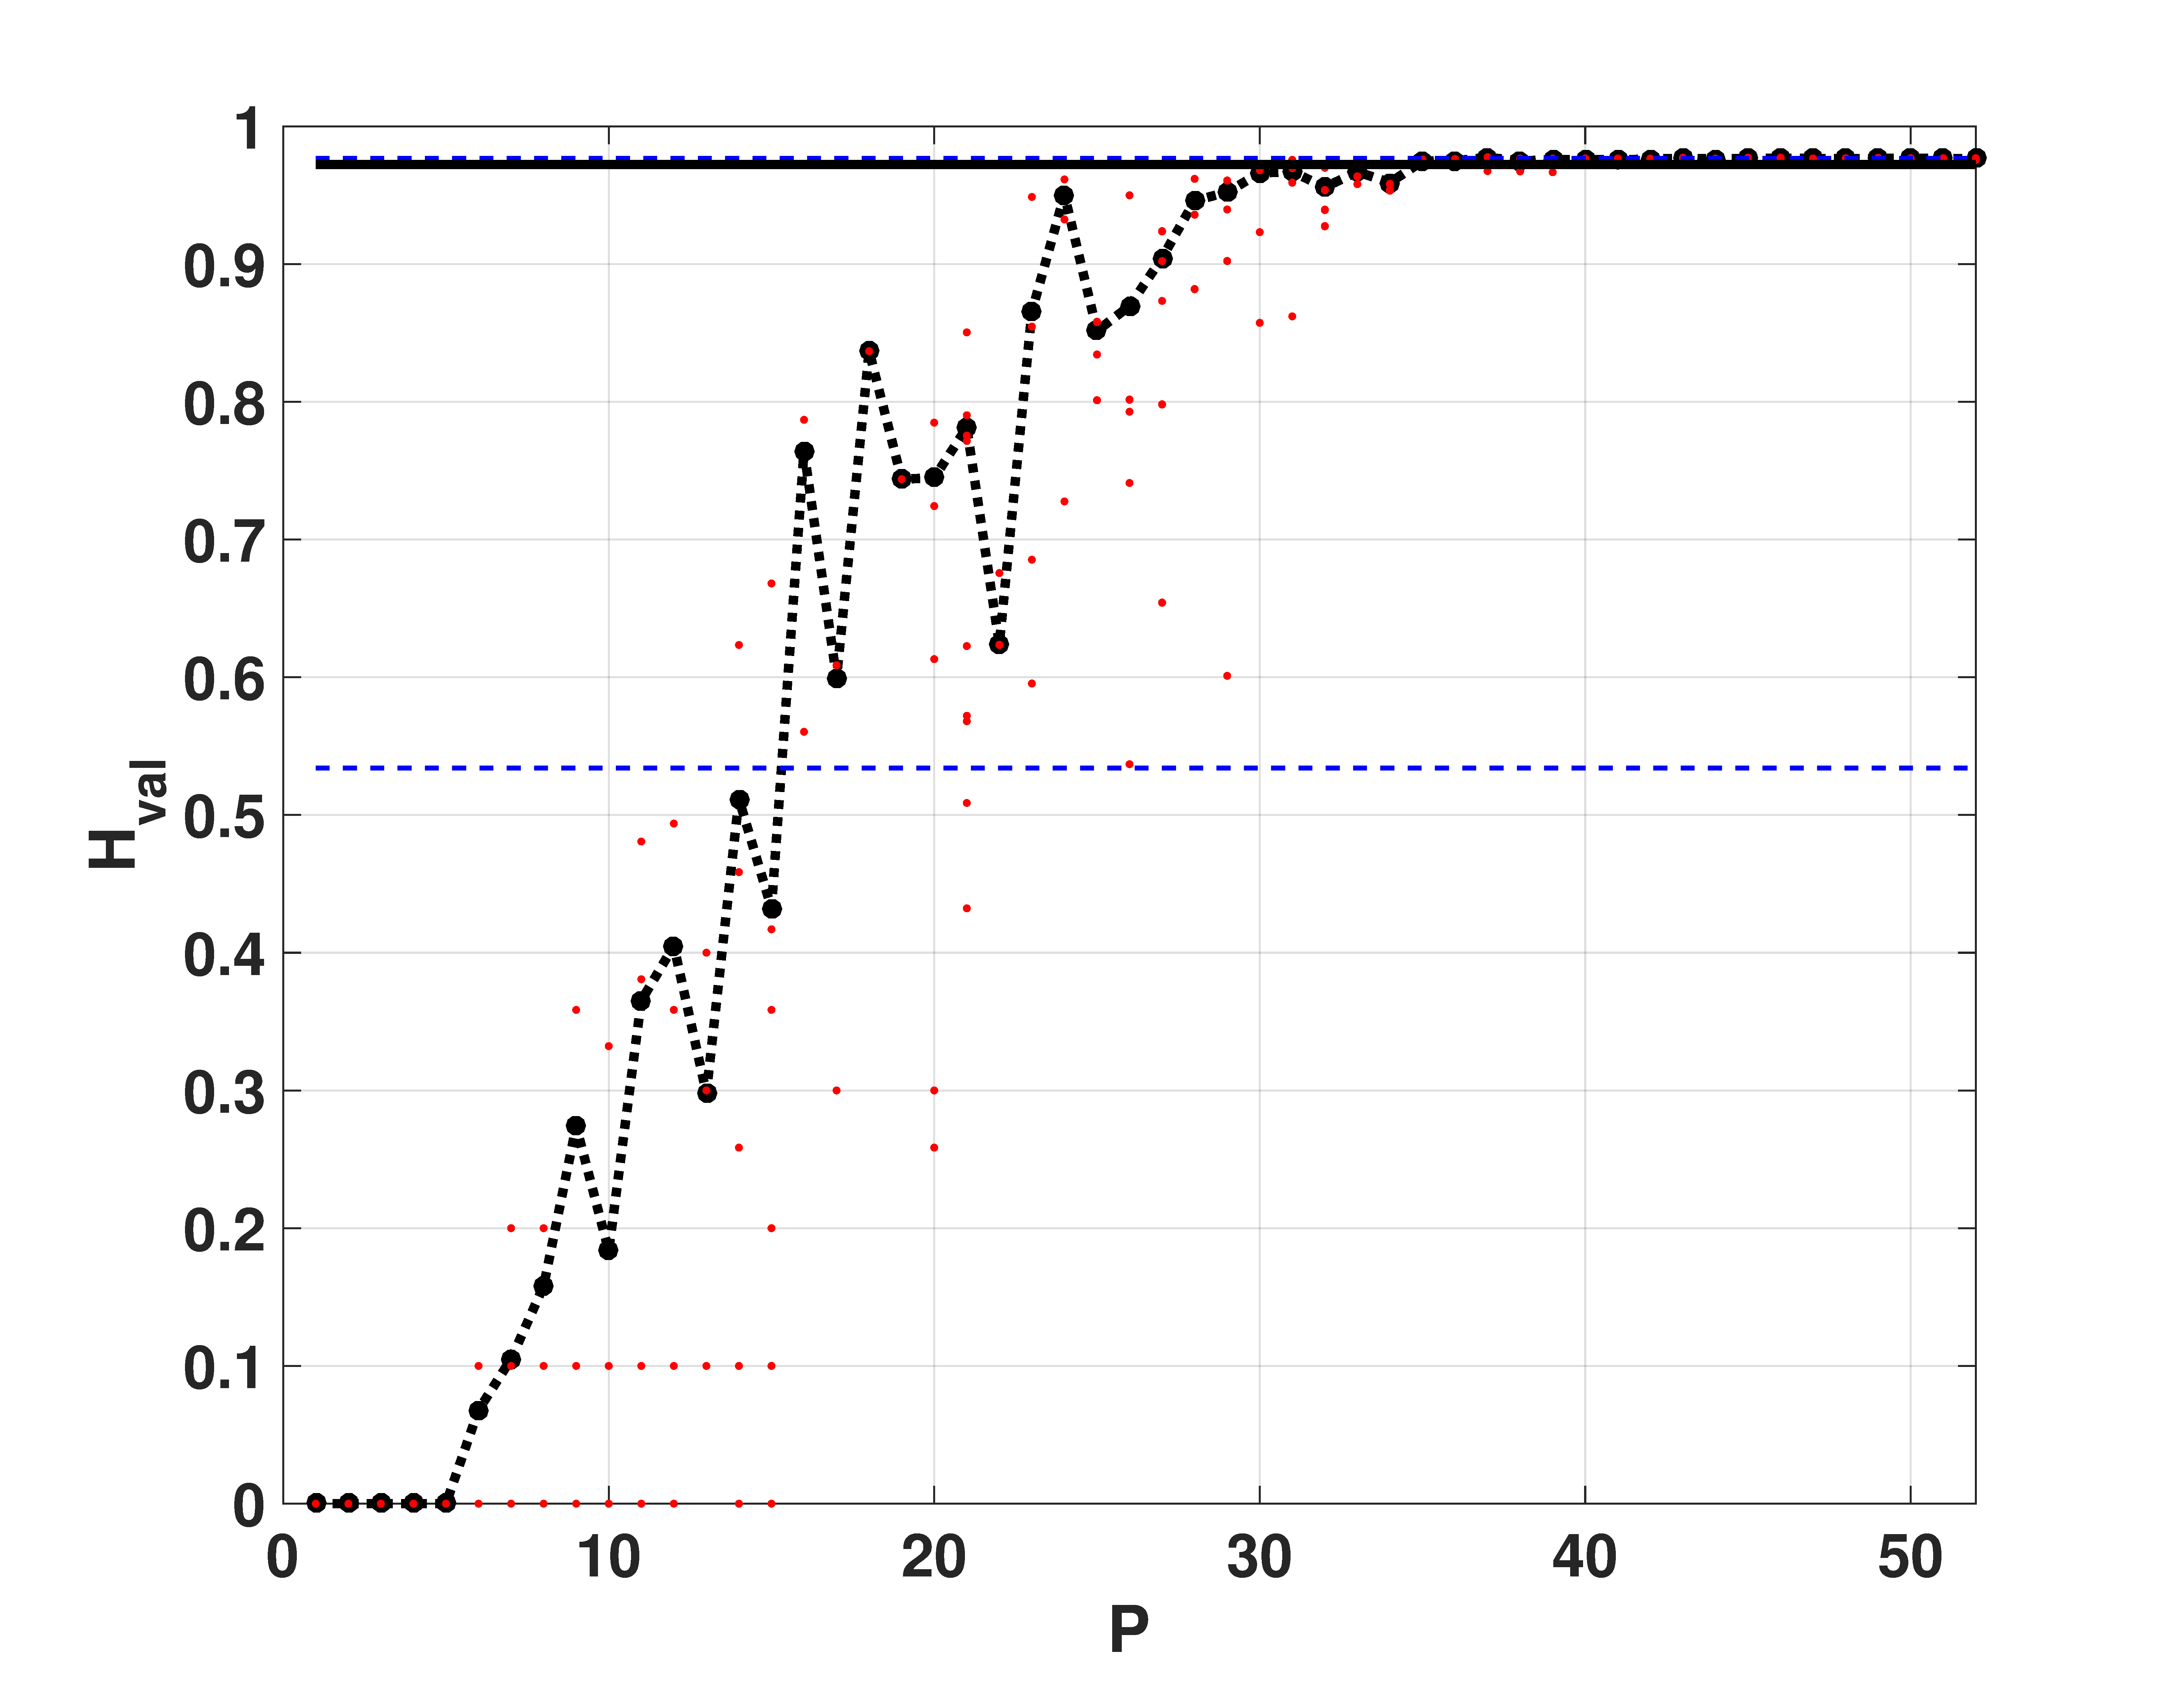
\includegraphics[width=.49\textwidth]{Hval_Switch}
	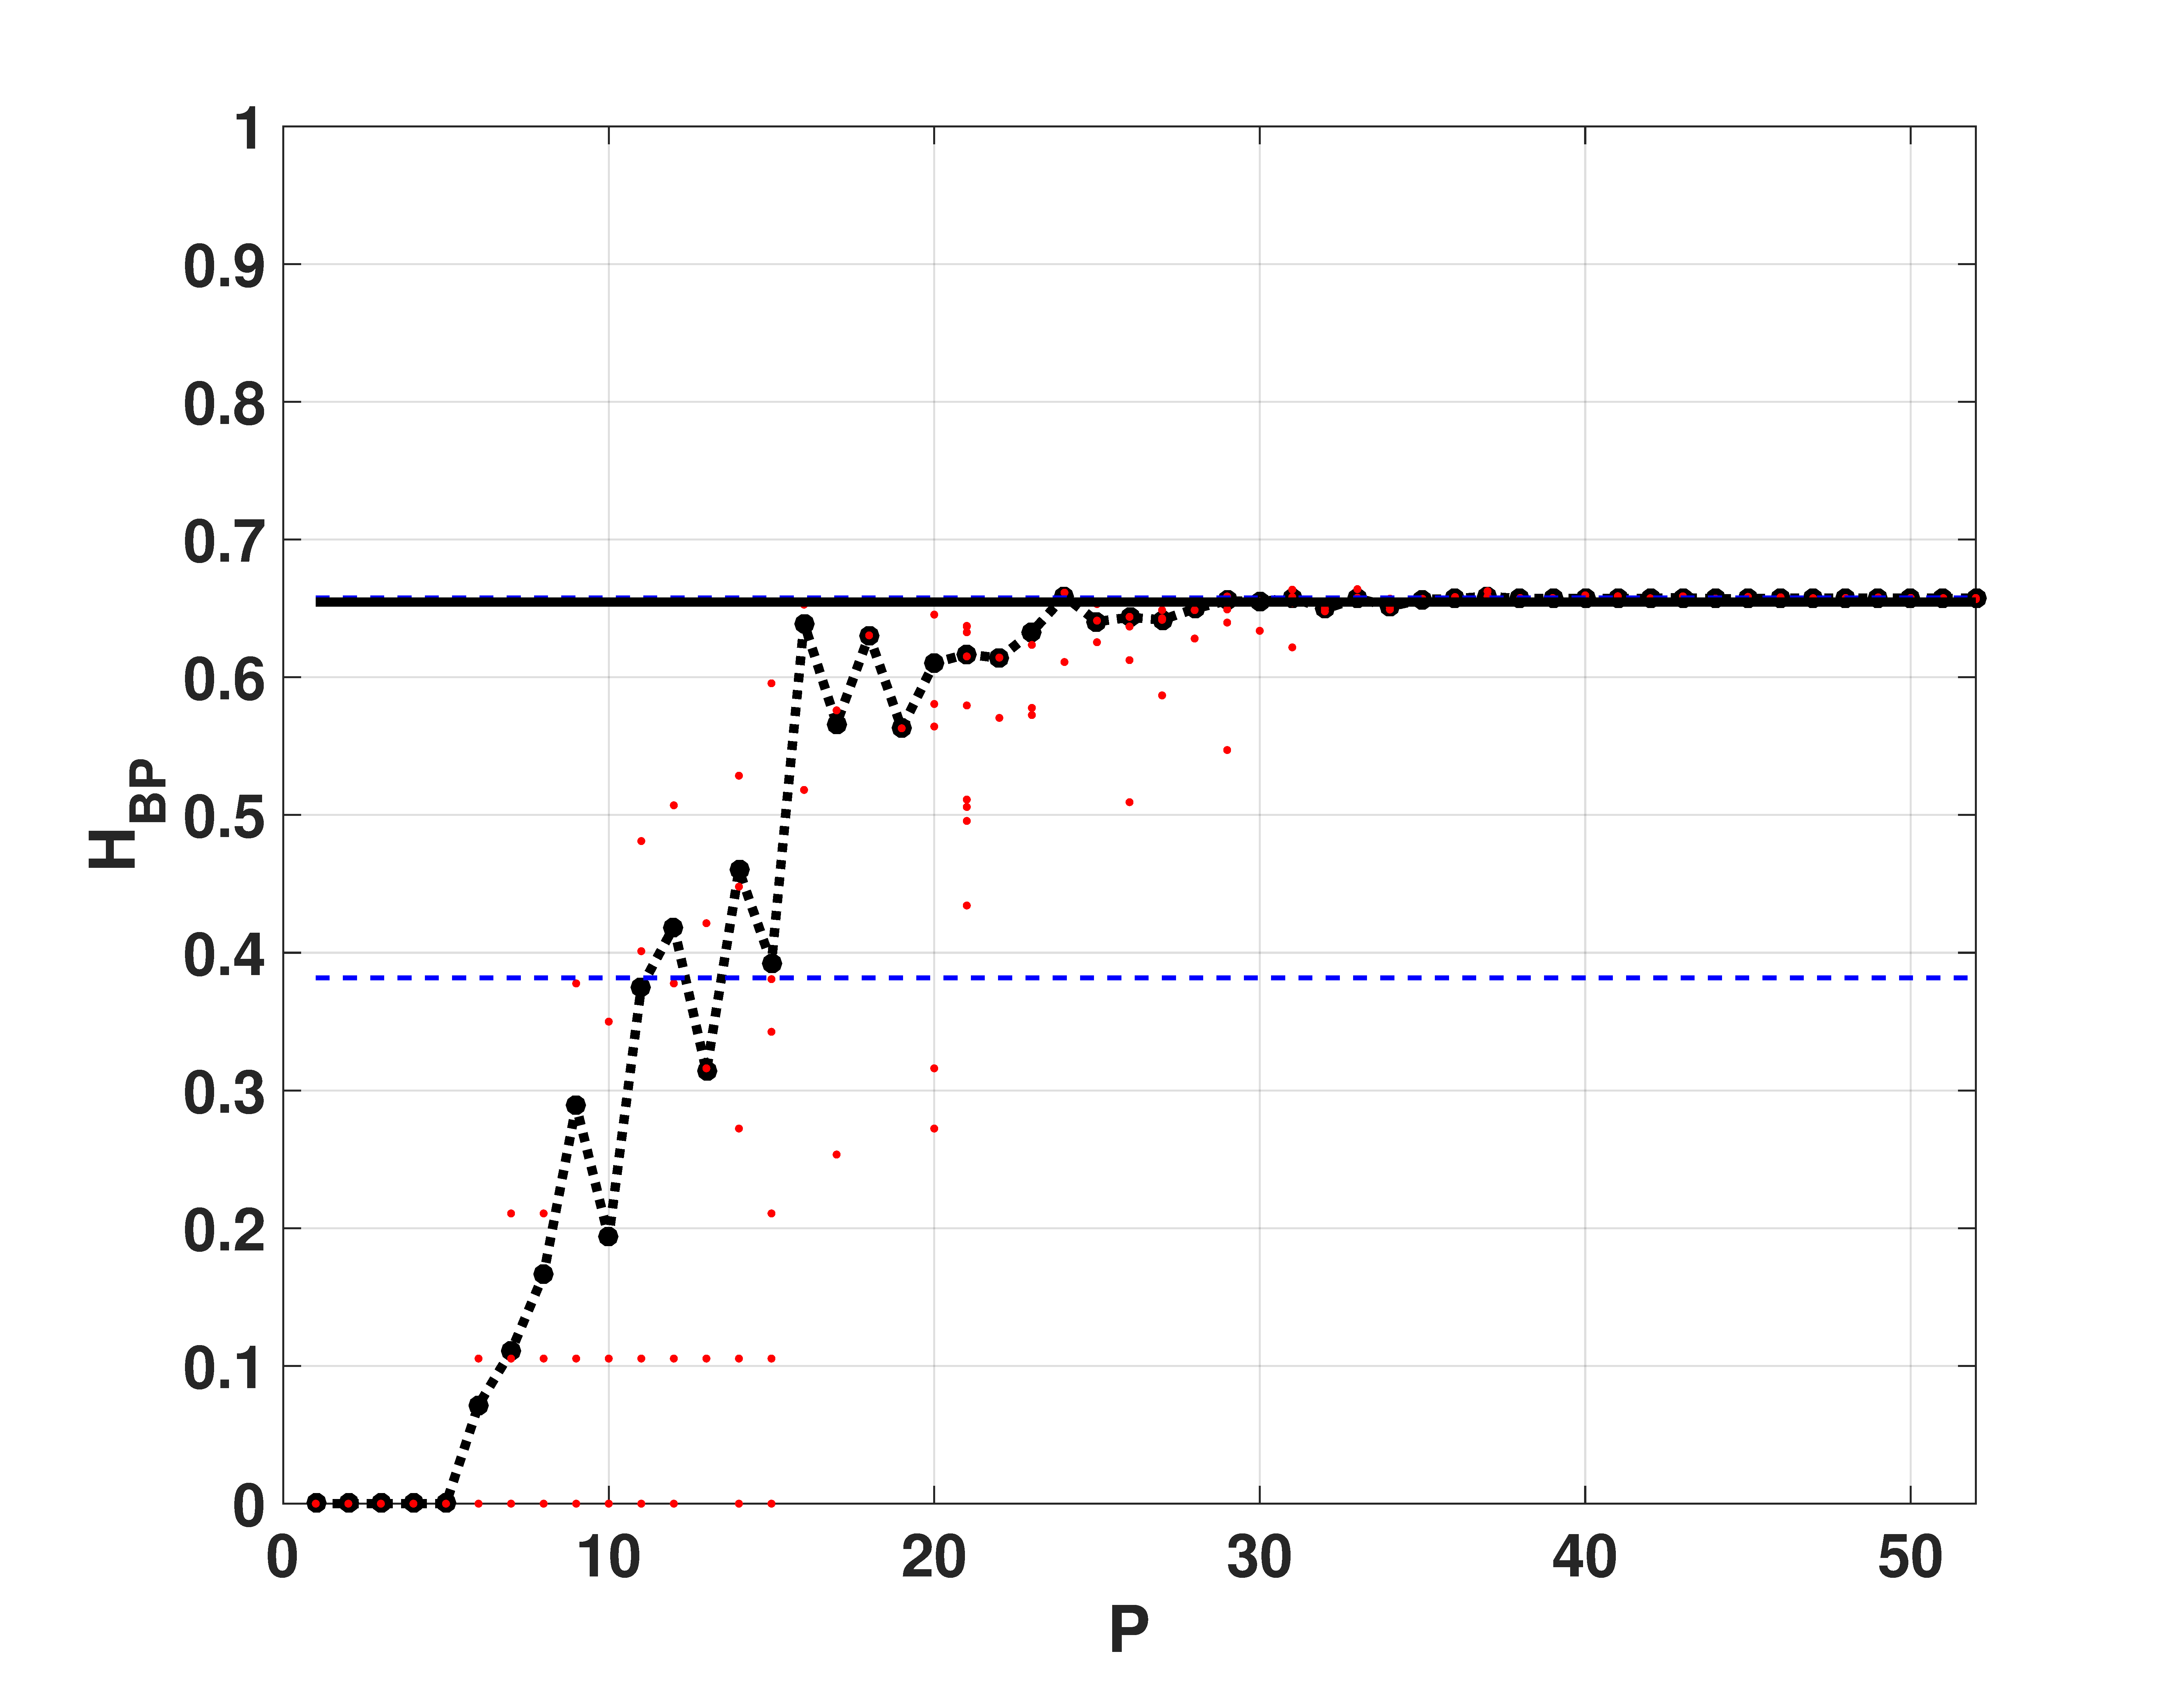
\includegraphics[width=.49\textwidth]{Hbp_Switch}
	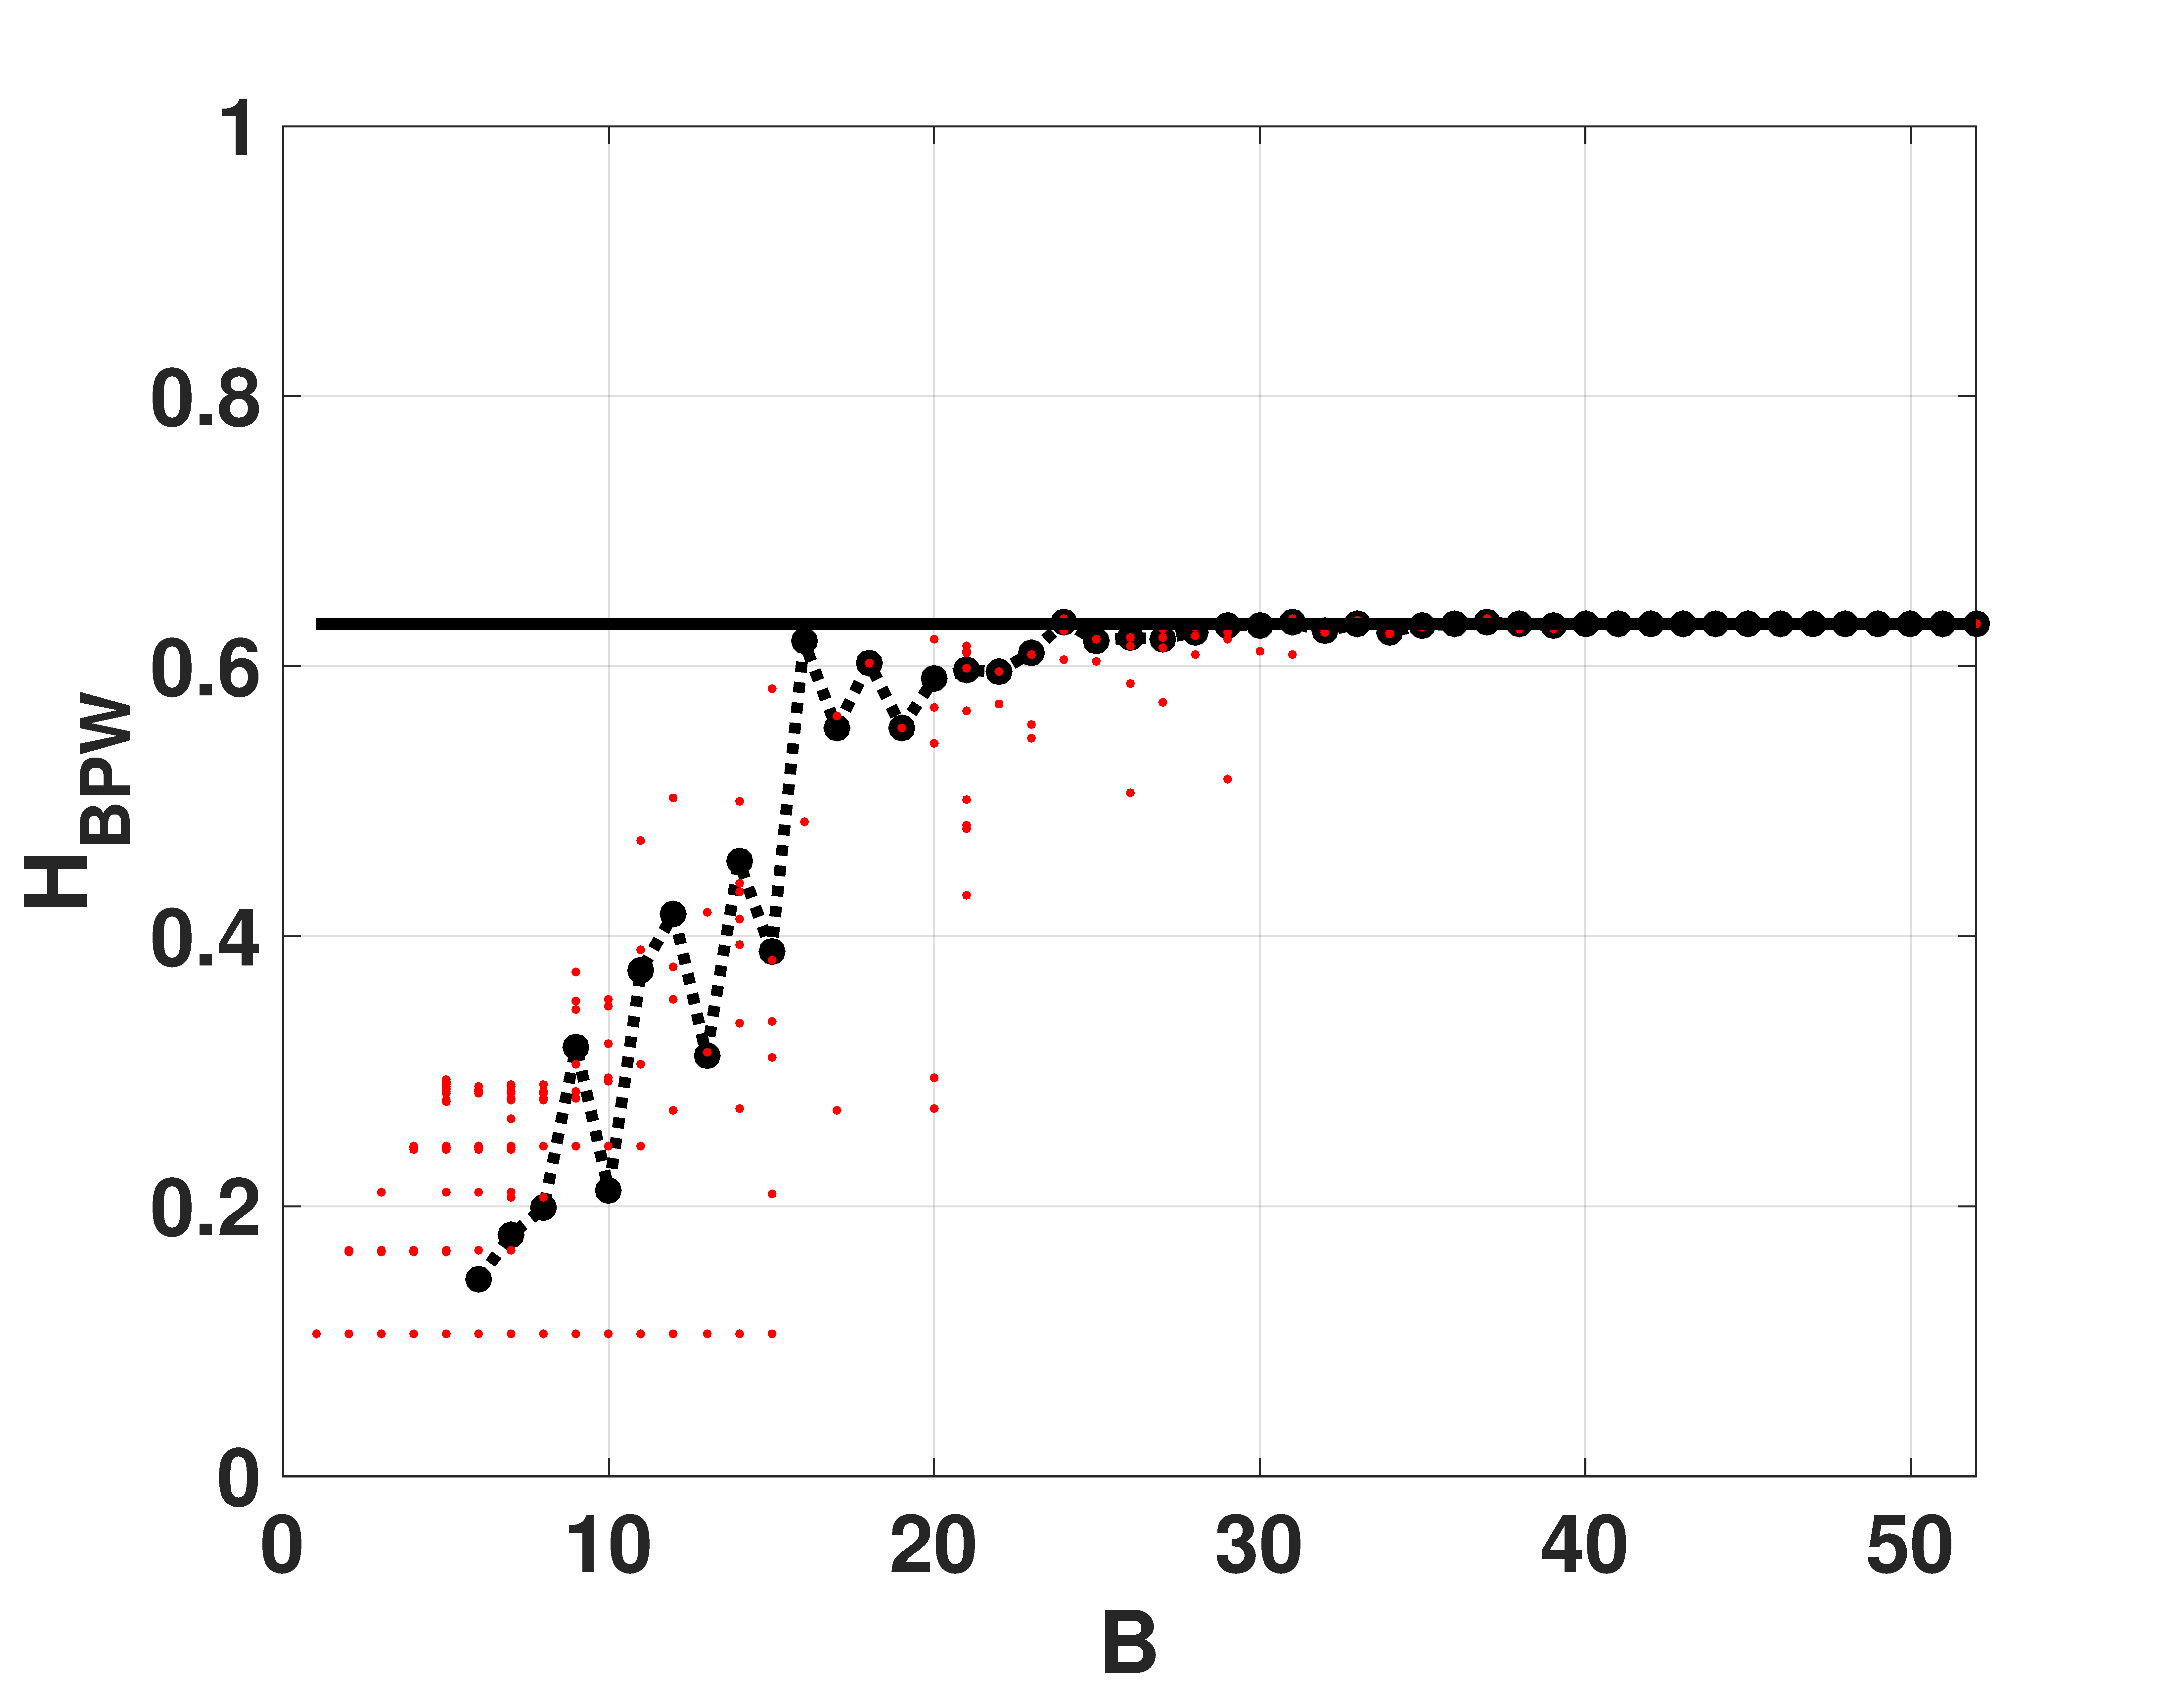
\includegraphics[width=.49\textwidth]{Hbpw_Switch}
	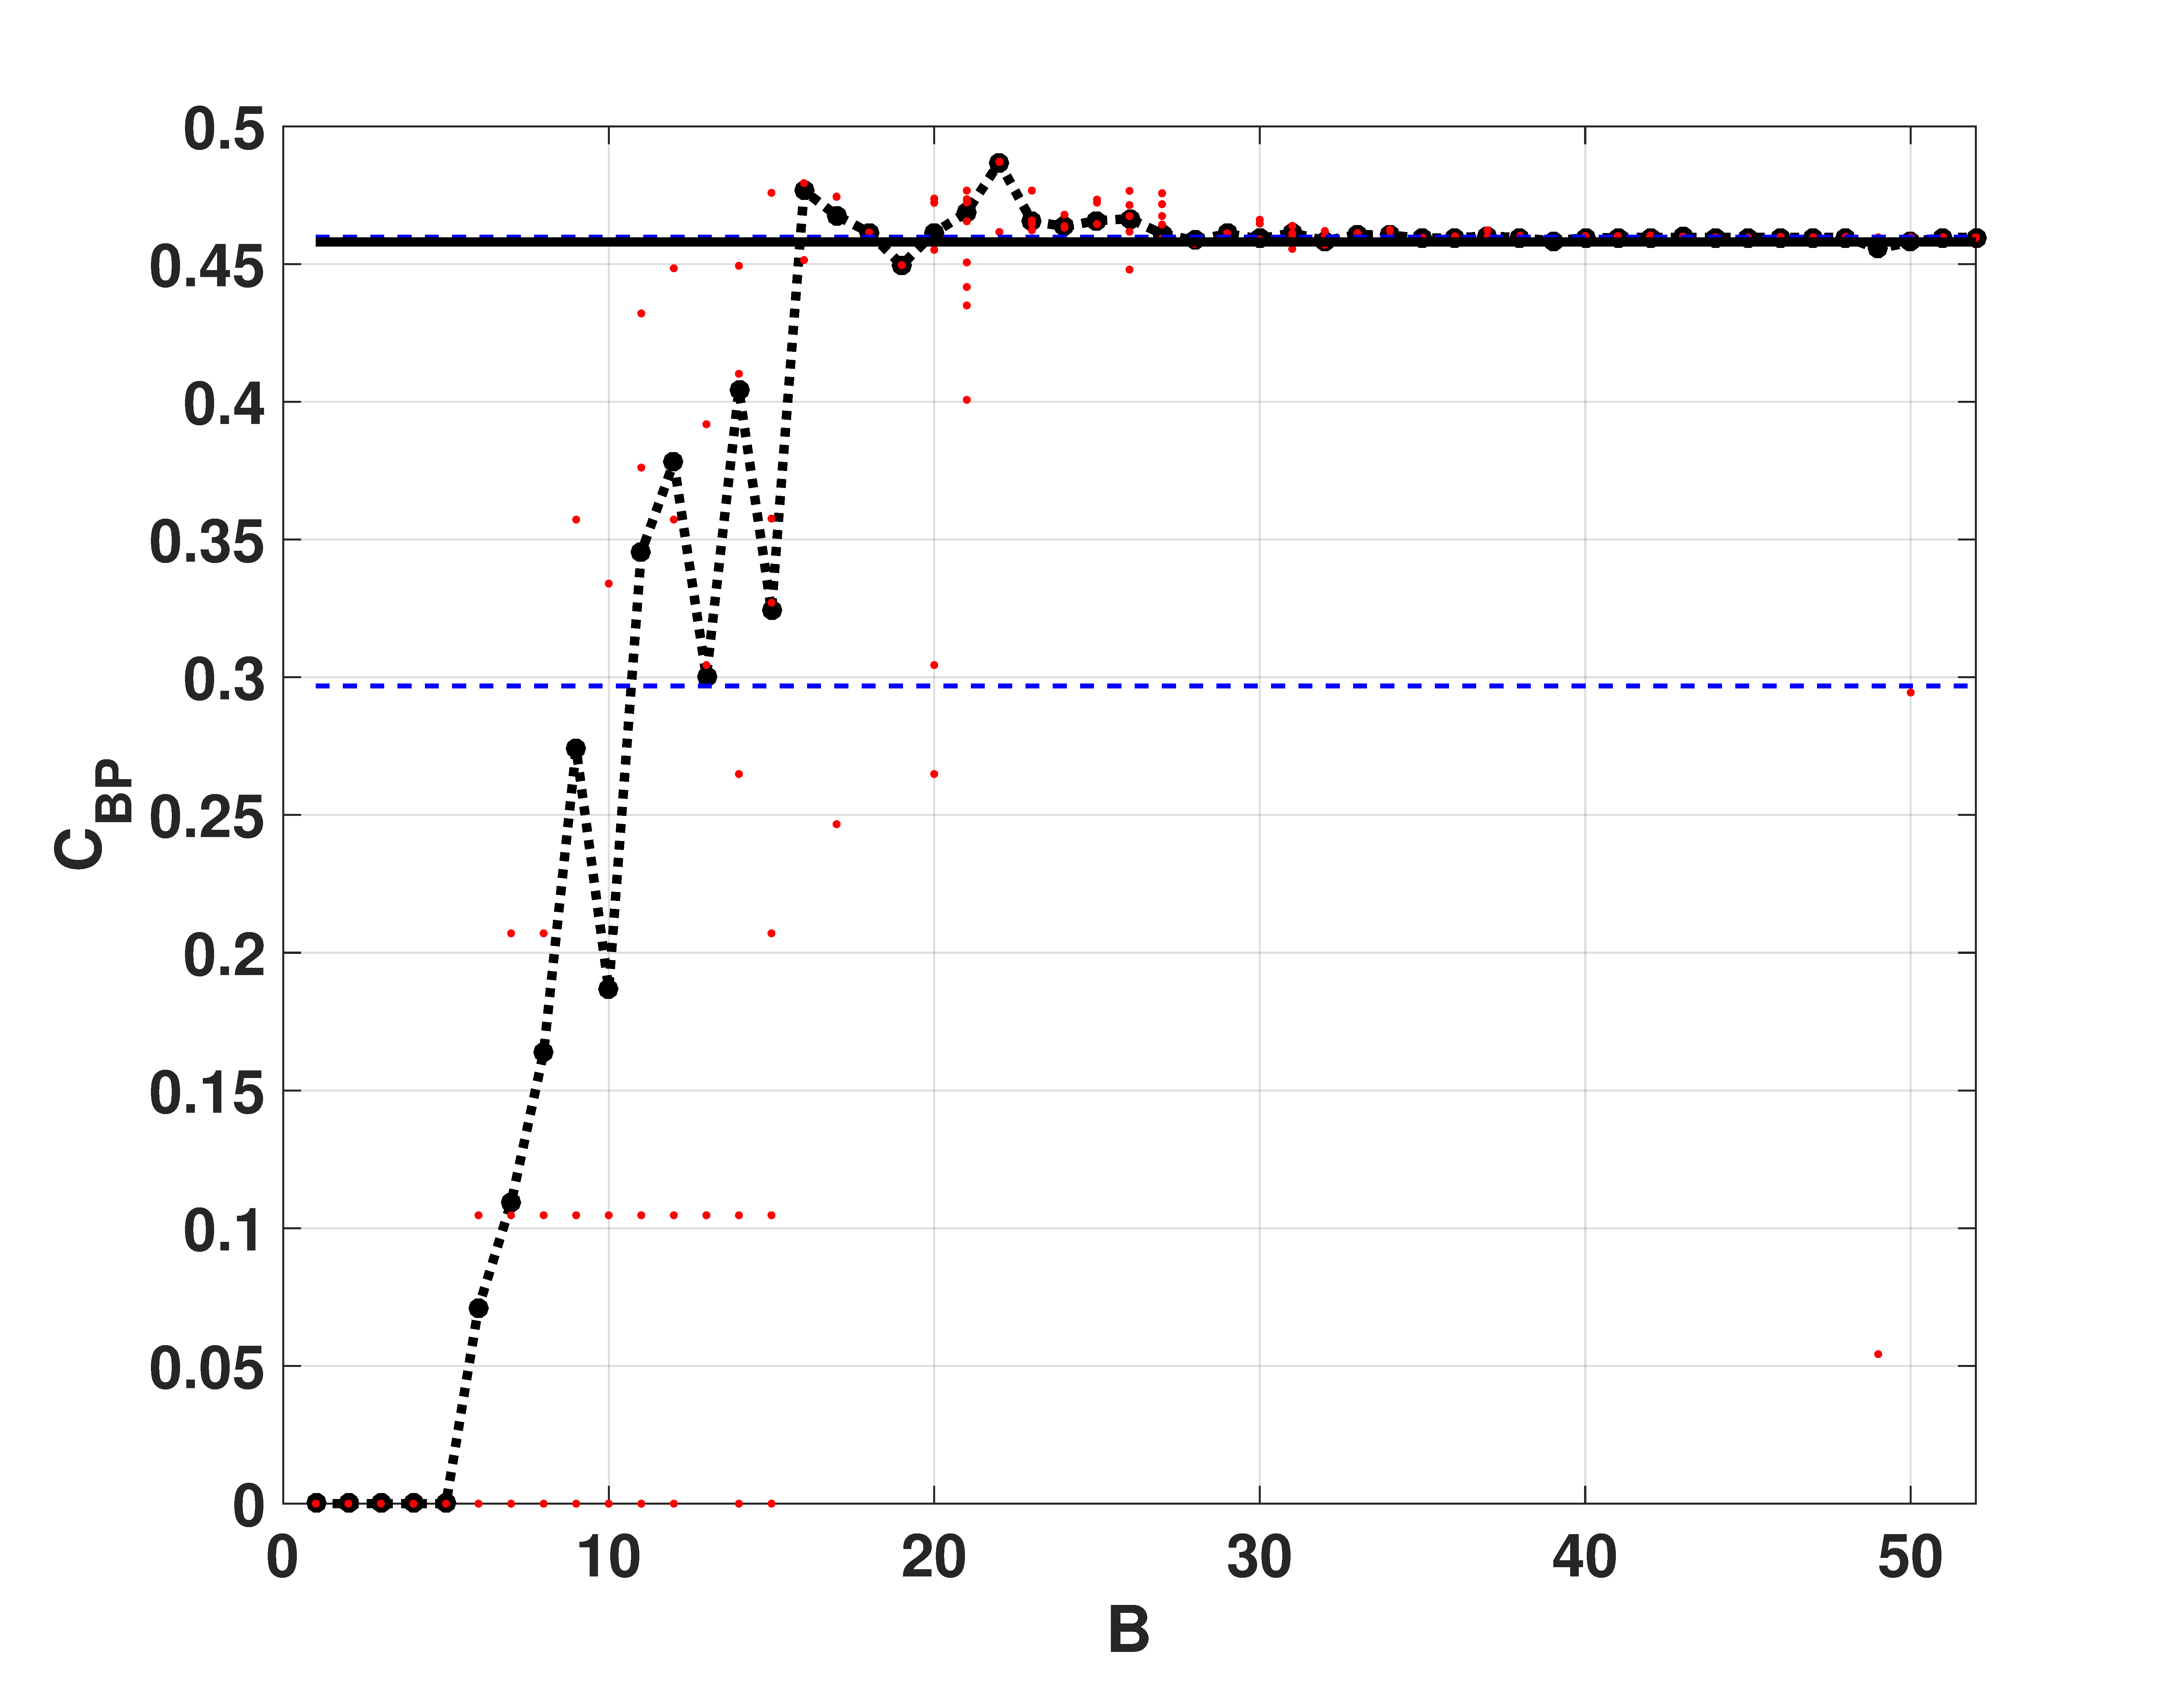
\includegraphics[width=.49\textwidth]{Cbp_Switch}
	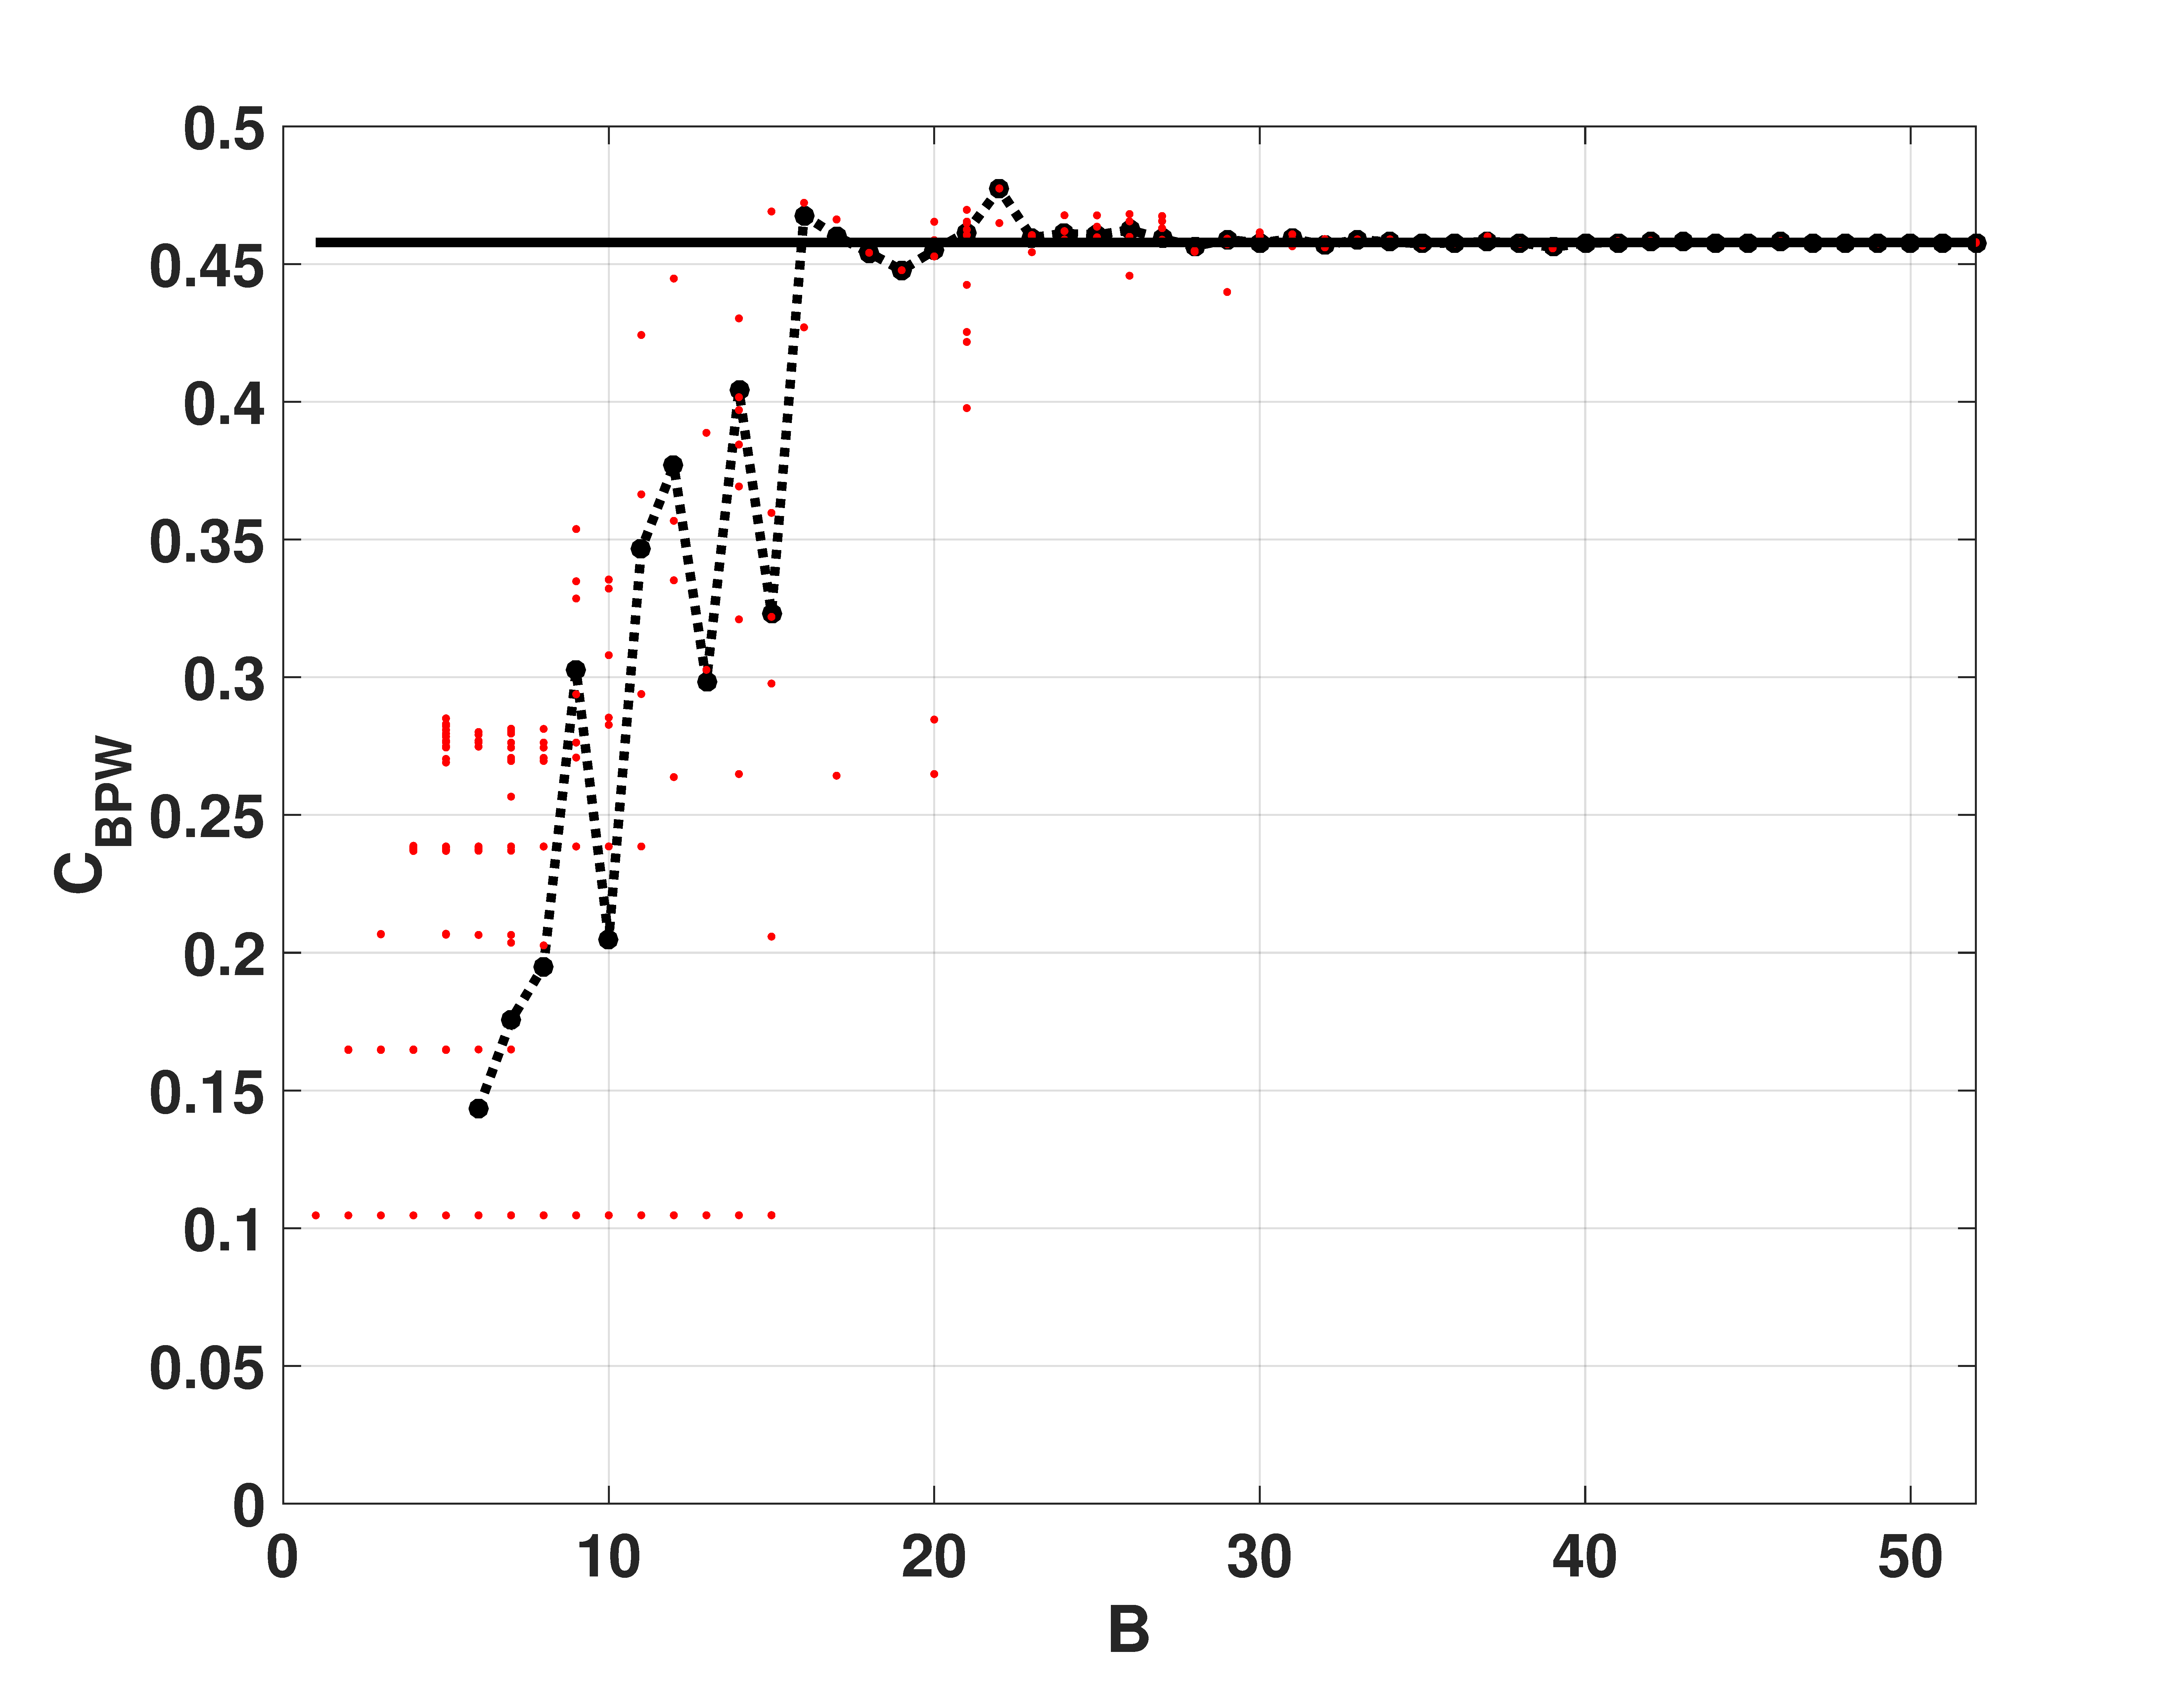
\includegraphics[width=.49\textwidth]{Cbpw_Switch}
	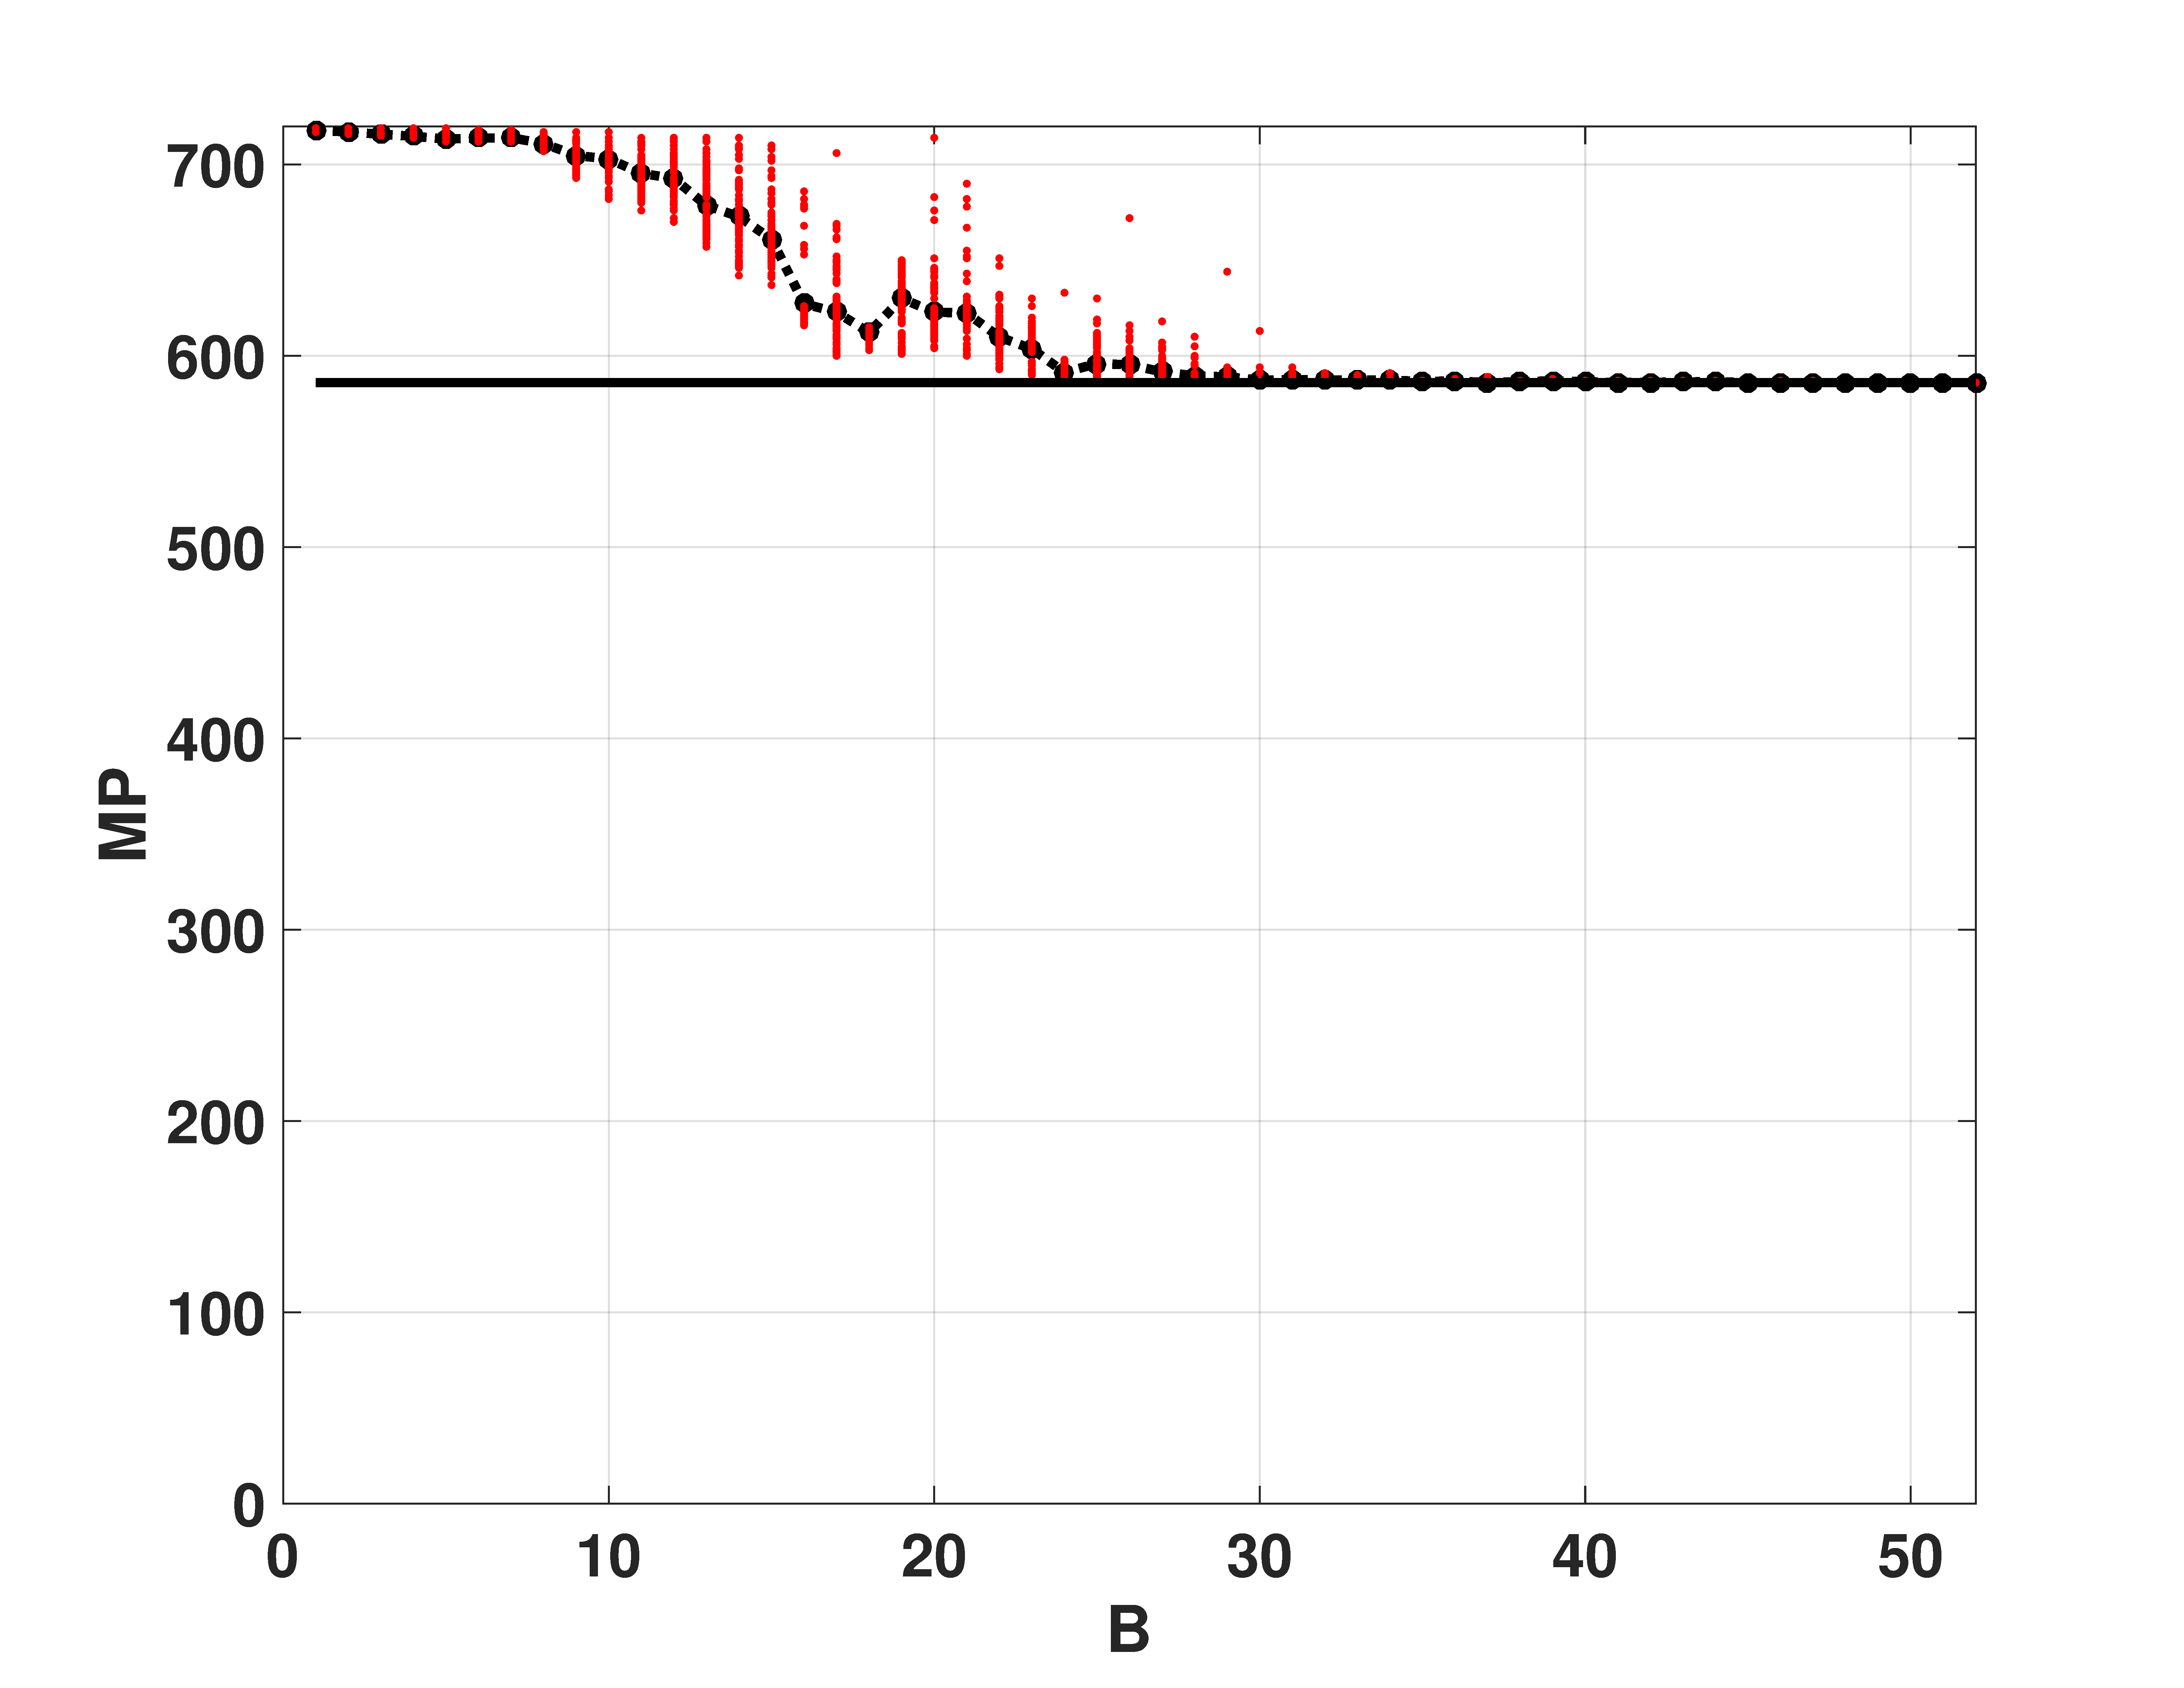
\includegraphics[width=.49\textwidth]{MP_Switch}
	\caption{Statistical properties of the SWITCH map: (a) $H_{val}$ vs $B$ (b) $H_{BP}$ vs $B$ (c) $C_{BP}$ vs $B$ (d) $MP$ vs $B$.}
	\label{fig:SWITCH_QuantiB}
\end{figure}

Double entropy plane $H_{val}$ vs $H_{BP}$ is showed in Fig. \ref{fig:SWITCH_HH}.
The point reached in this plane for SWITCH map is similar to that reached for LOG map.
The mixing is slight better in this case.

\textcolor{red}{TENDRÍA QUE SACAR MAS CONCLUSIONES DE LOS PLANOS TENDRÍA QUE VERLAS EN LAS SERIES DE DATOS, ESPECIALMENTE EL PUNTO ESE QUE DA CORRIDO}

\begin{figure}
	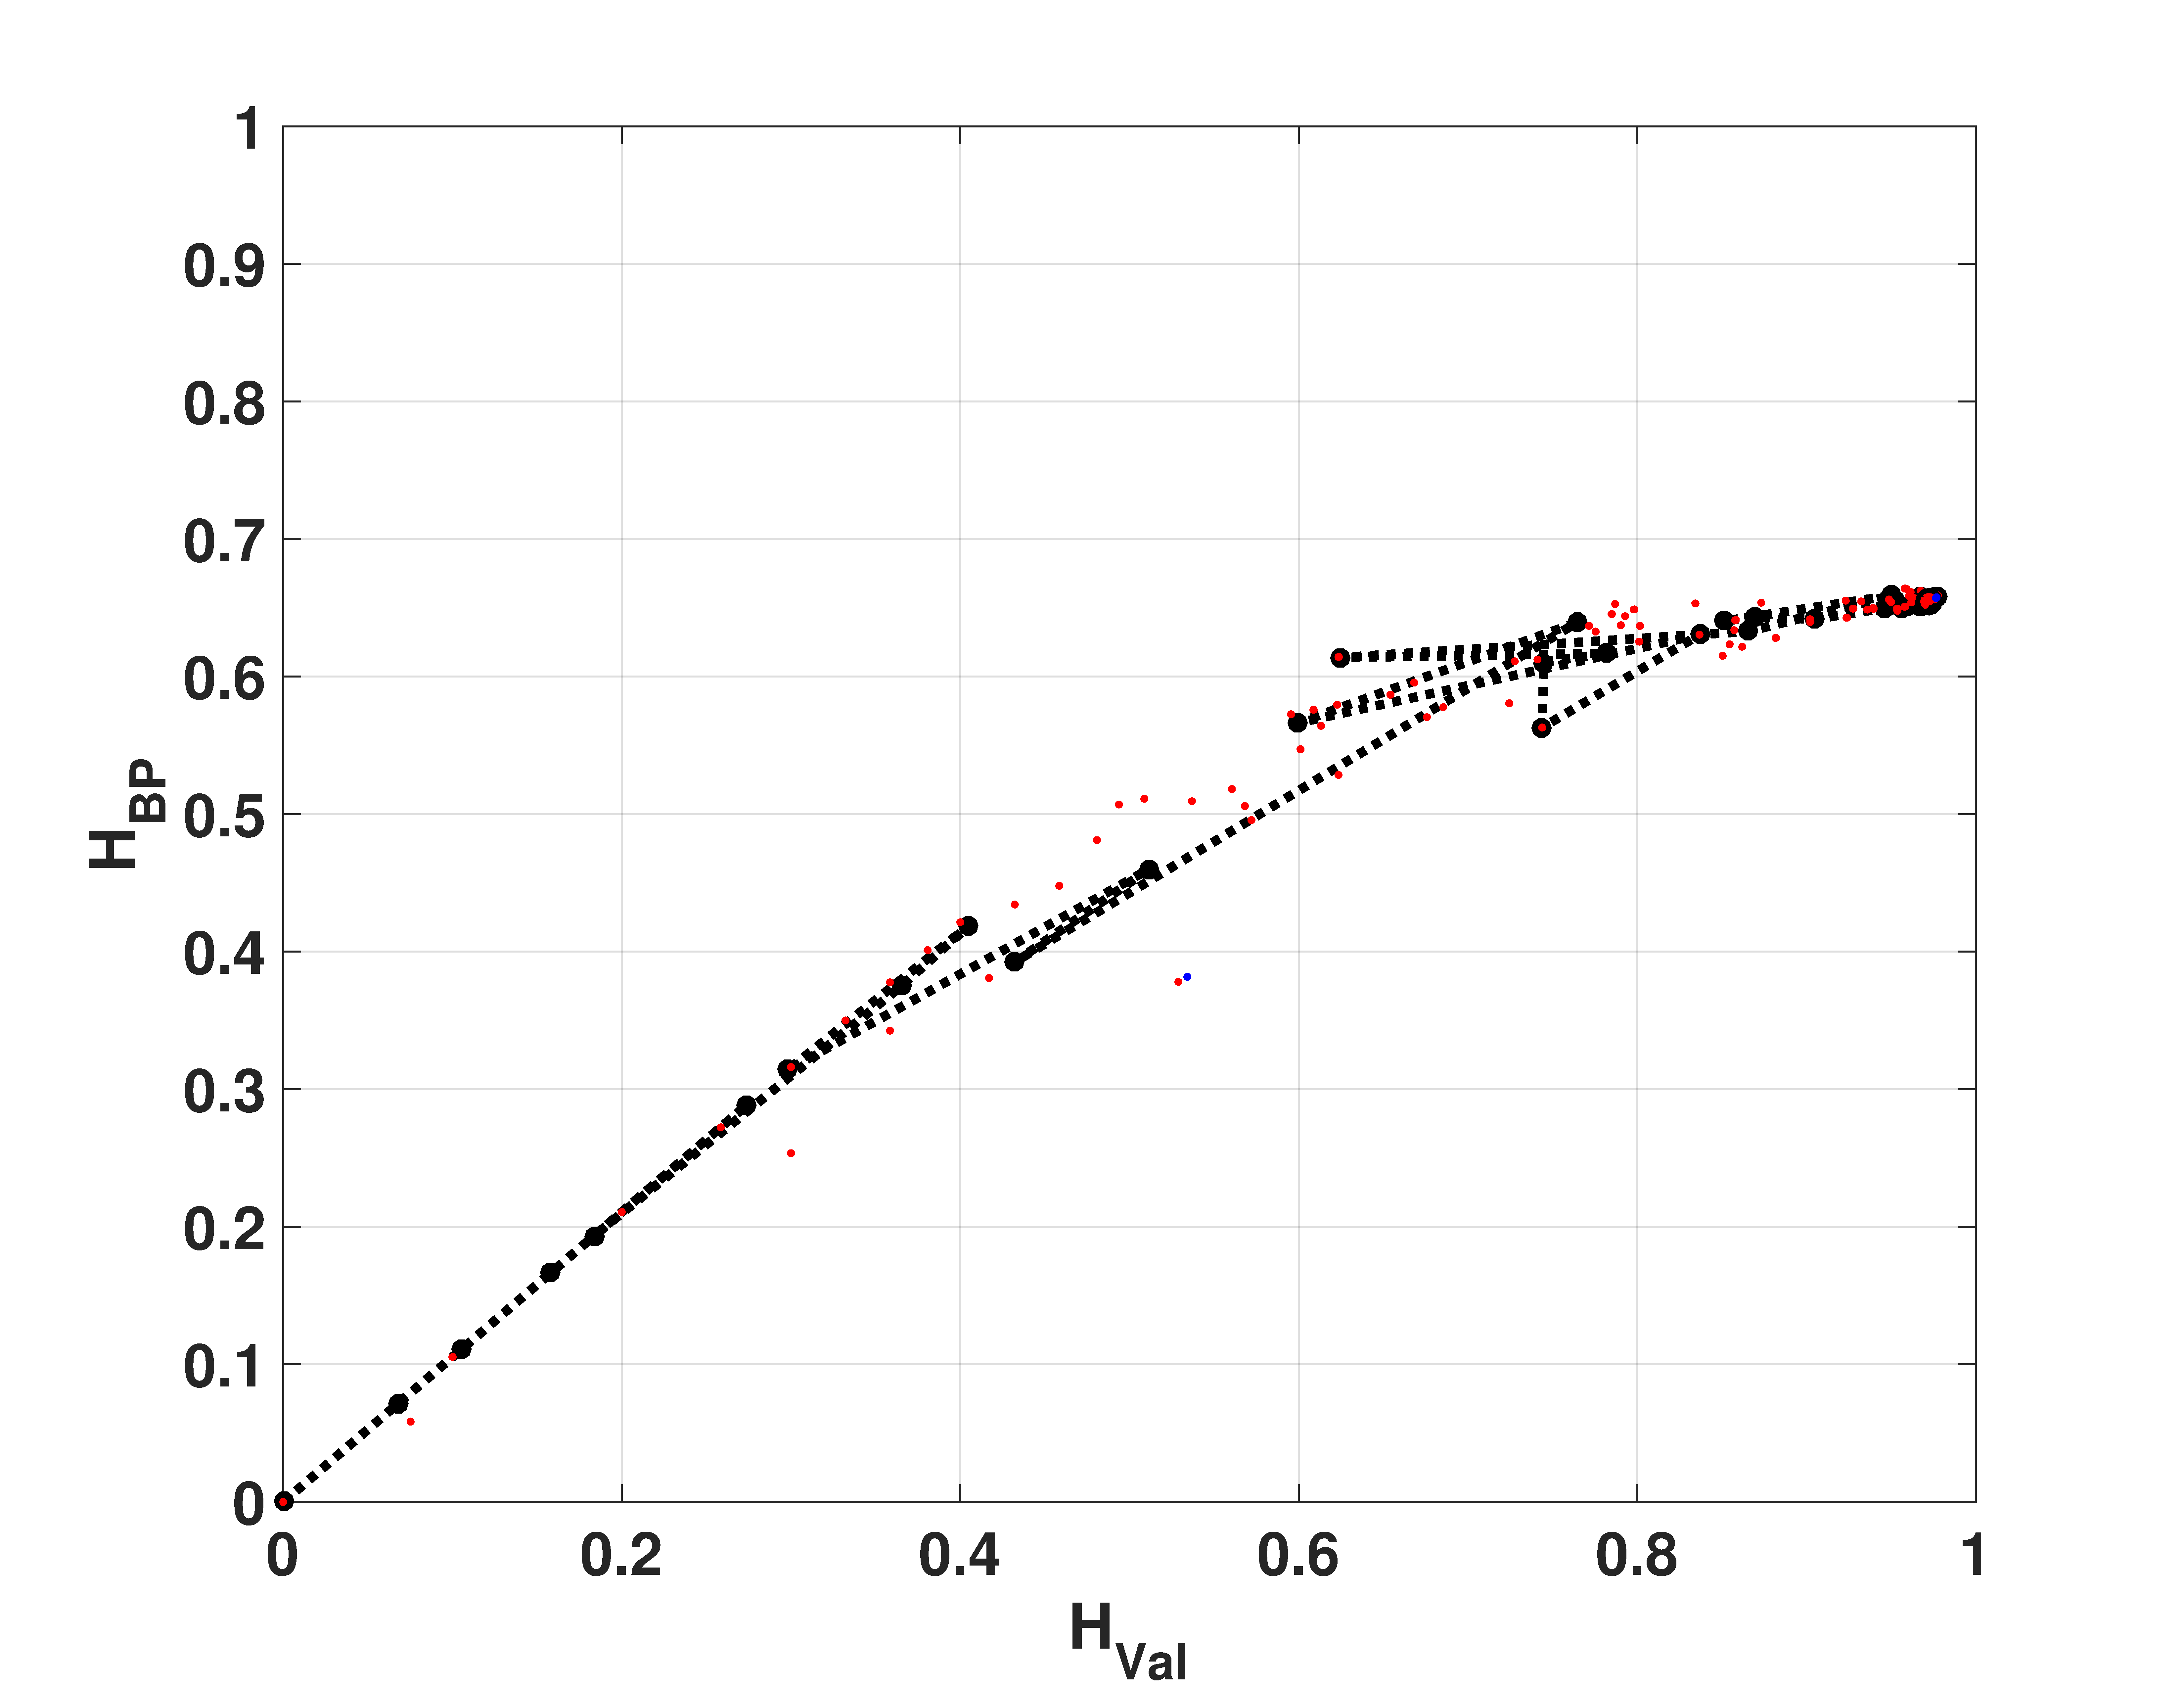
\includegraphics[width=.49\textwidth]{HbpHval_Switch}
	\caption{Evolution of statistical properties in double entropy plane of SWITCH map $H_{val}$ vs $H_{BP}$.}
	\label{fig:SWITCH_HH}
\end{figure}

Entropy-complexity plane $C_{BP}$ vs $H_{BP}$ is showed in Fig. \ref{fig:SWITCH_HC}.
If we compare with the same plane in the case of LOG (Fig. \ref{fig:LOG_HC}. a.), $C_{BP}$ is lower for SWITCH, this fact shows a more random behaviour.

\begin{figure}
	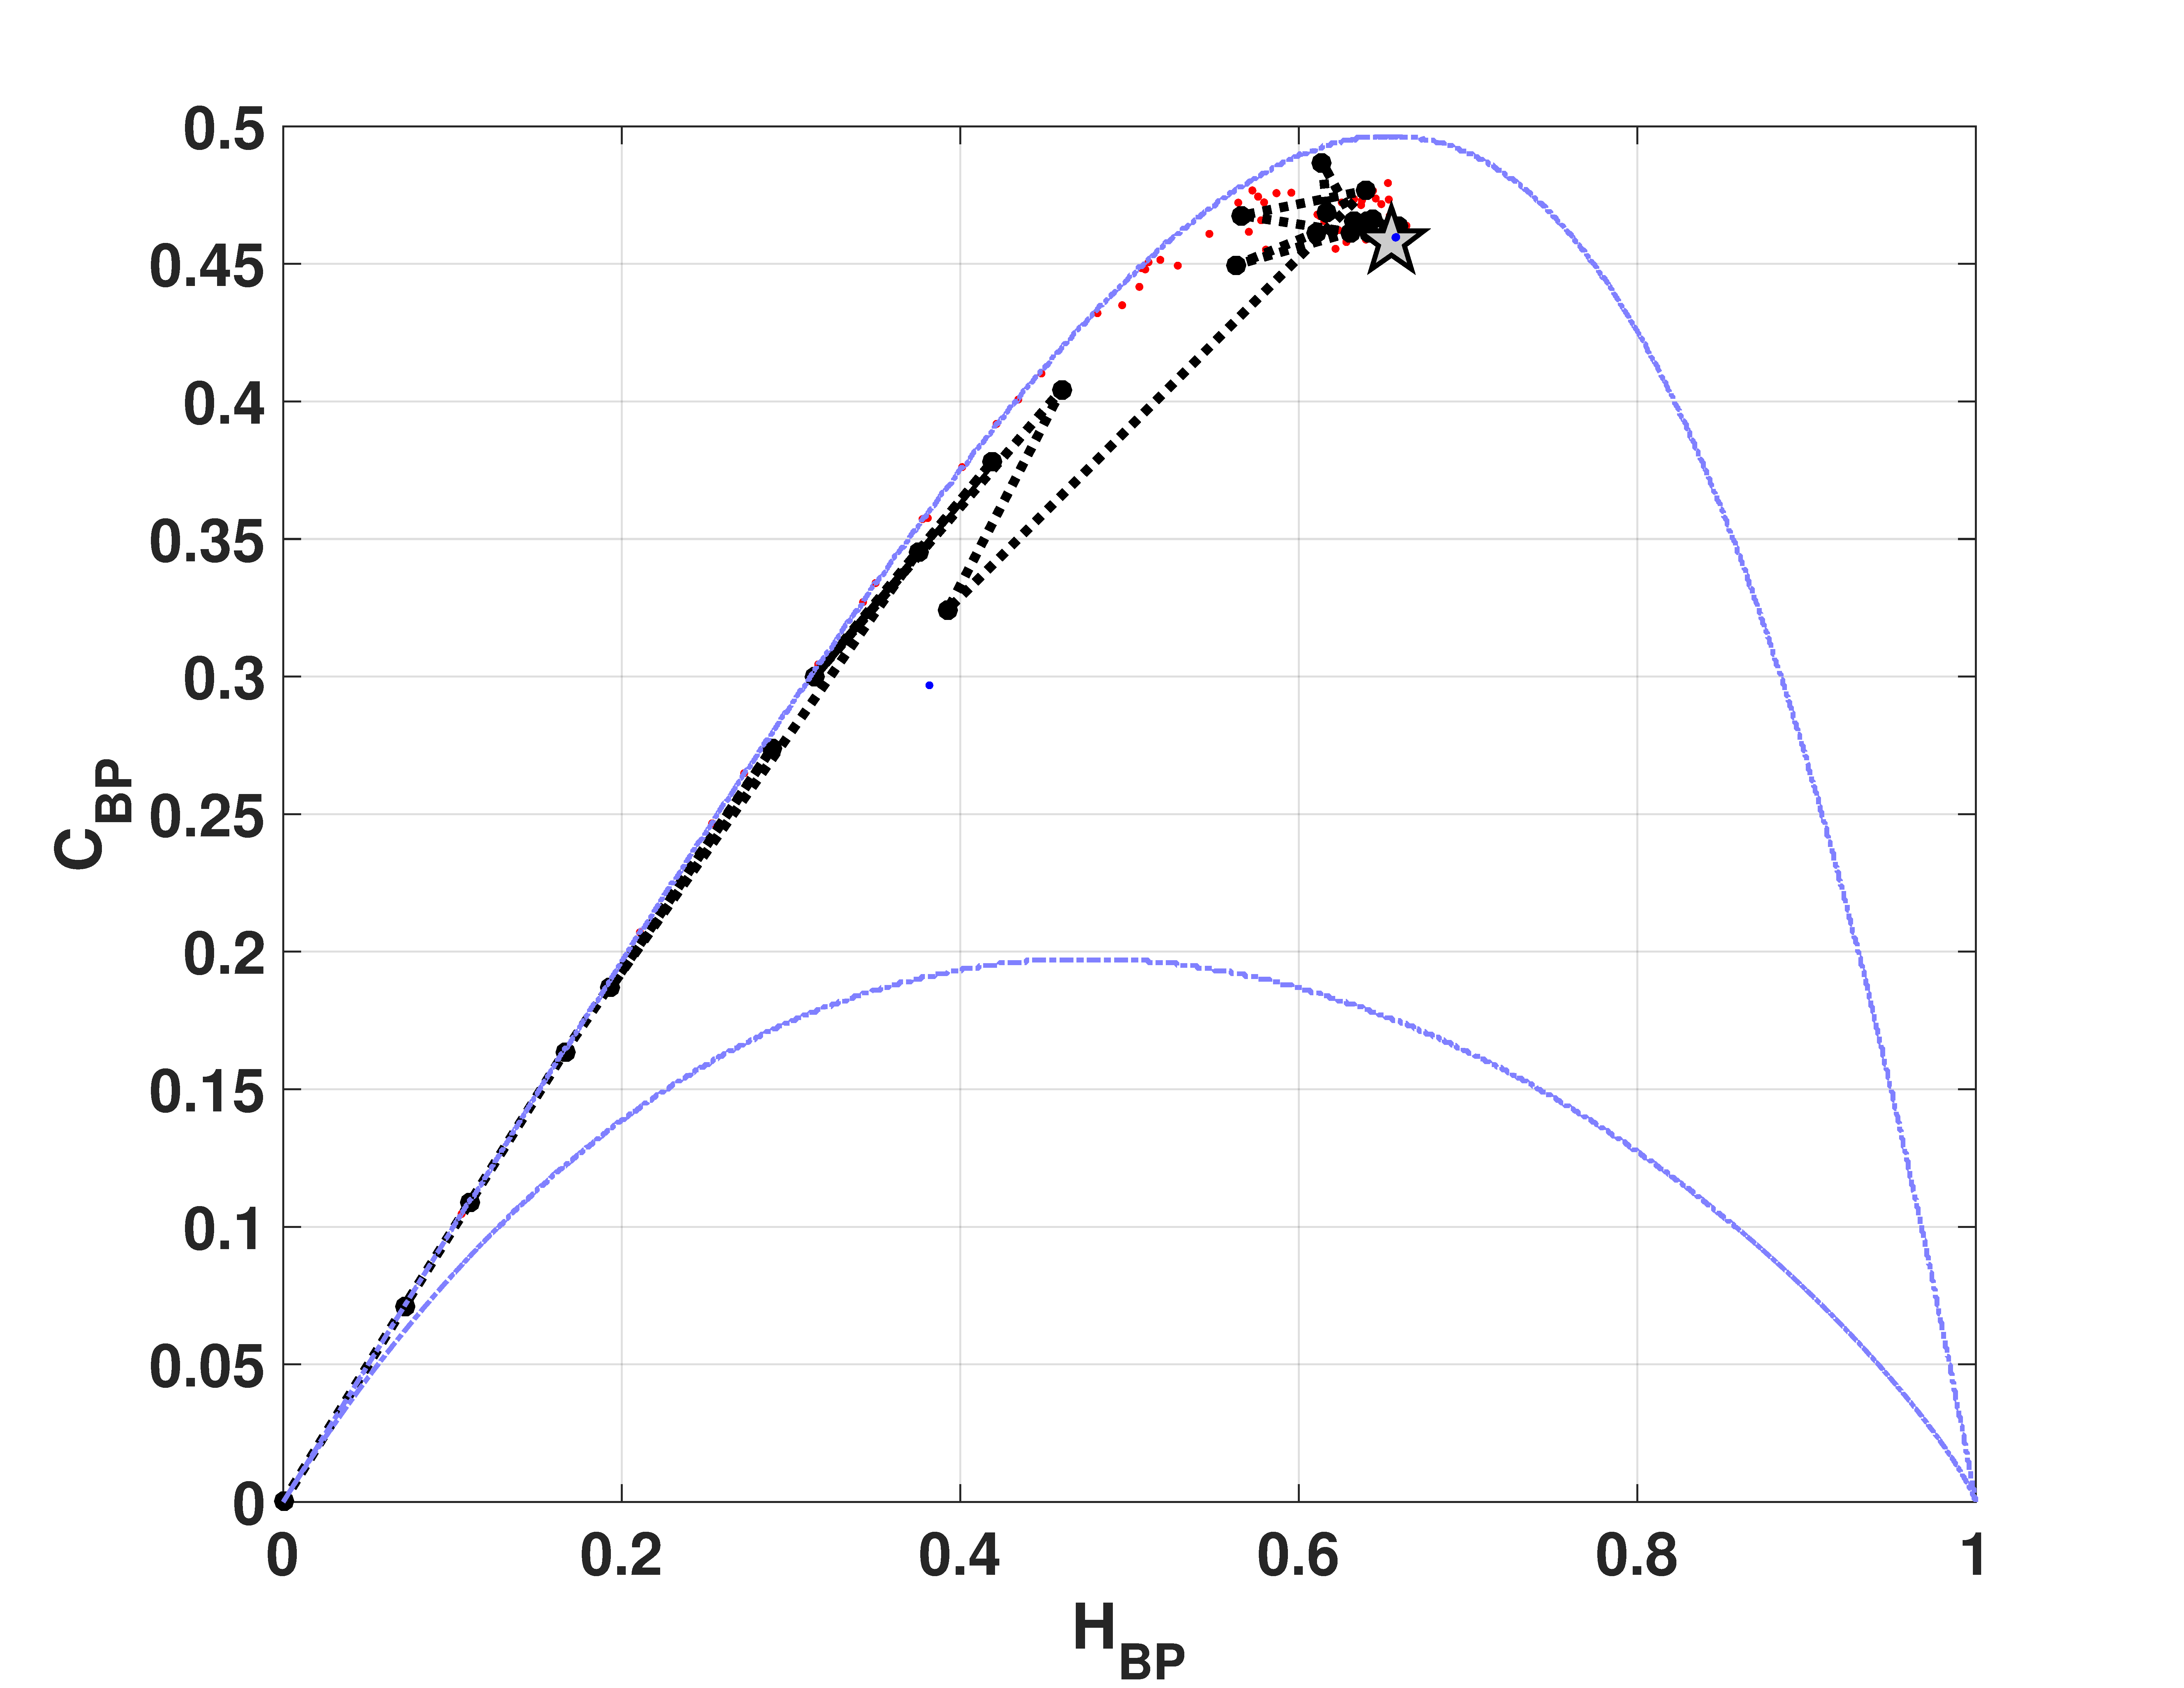
\includegraphics[width=.49\textwidth]{CbpHbp_Switch}
	\caption{Evolution of statistical properties in entropy-complexity plane of SWITCH map $C_{BP}$.}
	\label{fig:SWITCH_HC}
\end{figure}